\documentclass[twocolumn]{article}

\usepackage{tikz}
\usepackage{amsmath}
\usepackage{csquotes}
\usepackage{booktabs}
\usepackage{biblatex}
\usepackage[plain]{fancyref}

\usepackage{pgfplots}
\pgfplotsset{compat=newest}

\addbibresource{closedSetSpeakerVerification.bib}

\title{Closed Set Speaker Verification}

\author{
  Basant Mahgoub (20180162), Omar Emara (20180364), Hamza Mahmoud(20180214) \\
  Tarik Zaki (20180300), Habiba Yasser (20180188), Mohamed Alkhateb (20180470) \\
  Karim Ashraf (20180424), Mohamed AbdAllah (20180517)
}

\begin{document}

\maketitle

\begin{abstract}

  Closed set speaker verification is a type of speaker recognition where the
  system verifies a certain identity claim in a form of a voice sample by
  comparing it with a finite set of stored models representing different
  voice-prints. We present a machine learning model for speaker verification
  based on a voice samples dataset. In \Fref{sec:Introduction}, we introduce the
  concept of speaker verification and the detection mechanism. In
  \Fref{sec:Dataset}, we present the dataset, discuss the utilized feature
  extraction method, and define the final form of the generated features. In
  \Fref{sec:Implementation}, we present a binary classifier implementation using
  both artificial neural networks and support vector machine models. In
  \Fref{sec:Results}, we present the results of each of the implementations.
  Finally, we conclude in \Fref{sec:Conclusion}.

\end{abstract}

\section{Introduction}
\label{sec:Introduction}

\emph{Speaker Verification} systems are systems that can verify a certain
identity claim. Those systems are sometimes called one to one speaker
recognition. In those systems, one makes a claim that one is a certain person
providing a voice sample as a proof of the claim. The system then compares this
voice sample with a stored \emph{model} or \emph{template} that the system
previously generated. Finally, the system either accepts or rejects the claim. A
closed set system guarantees that the input voice sample belongs to a person
known to the system at training time. The main application for this system is
access control systems, where the verification is used to grant access to a
certain resource.

The architecture of a traditional speaker verification system is illustrated in
\Fref{fig:SystemArchitecture}. Essentially, once a voice sample is input into
the system, the system extracts useful \emph{features} from the input and
matchs those features with the models it already has stored. Finally, the
system makes a decision in the form of a claim verification.

\begin{figure}
\begin{center}
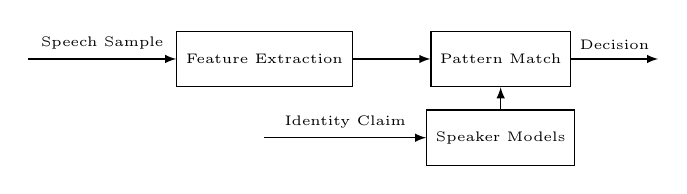
\begin{tikzpicture}[auto, node distance = 3cm, > = latex, font = \tiny]
\tikzset{
  block/.style = {draw, fill = white, rectangle, minimum height = 2em},
  input/.style = {coordinate},
  output/.style = {coordinate},
}
\node [input] (speechSample) {};
\node [block, right of = speechSample] (featureExtraction) {Feature Extraction};
\node [block, right of = featureExtraction] (patternMatch) {Pattern Match};
\node [block, below of = patternMatch, node distance = 1cm] (speakerModels) {Speaker Models};
\node [input, left of = speakerModels] (identityClaim) {};
\node [output, right of = patternMatch, node distance = 2cm] (decision) {};
\draw [->] (speechSample) -- node{Speech Sample} (featureExtraction);
\draw [->] (featureExtraction) -- (patternMatch);
\draw [->] (speakerModels) -- (patternMatch);
\draw [->] (identityClaim) -- node{Identity Claim} (speakerModels);
\draw [->] (patternMatch) -- node{Decision} (decision);
\end{tikzpicture}
\end{center}
\caption{The architecture of a general speaker verification system.}
\label{fig:SystemArchitecture}
\end{figure}

The feature extraction step is described in \Fref{sec:Dataset} and the pattern
matching step is described in \Fref{sec:Implementation}.

\section{Dataset}
\label{sec:Dataset}

We shall utilize the dataset provided in \autocite{Zohar2018} for developing the
models. The dataset contains 3000 English sound files voiced by 6 different
speakers. The files do not necessary have the same number of samples or the same
sample rate.

\subsection{Feature Extraction}

The system receives a digital sound signal, which is nothing more than a number
of samples sampled at different times at a certain rate called the
\emph{Sampling Rate}. It is very difficult to use this raw signal in pattern
matching, so a different representation of the signal is needed. The process of
finding this representation is called \emph{Feature Extraction}. We can broadly
classify the features we can extract into \emph{High-Level Features} and
\emph{Low-Level Features}.

\subsubsection{High-Level Features}

High-level features in the context of speech processing usually means
linguistic features. Such as the words used in the speech, the frequency of the
used words, the pauses that the speaker makes, and so on. Those features are
not very useful in most applications because they require long speeches to
extract meaningful information. Moreover, they are subject to voluntary
variations in speech. For instance, one can change the way one speaks to get
around speaker verification systems that matches high-level features.

\subsubsection{Low-Level Features}

Low-level features in the context of speech processing usually means acoustic
features. Acoustic features are intrinsic to the speech apparatus of the
speaker. So the speaker has little voluntary control over those features.
Moreover, it is possible to extract those features from small speech segments.
The most common low-level feature to extract is the \emph{Mel-Frequency
Cepstral Coefficients (MFCCs)}, which we shall introduce in the next section.

\subsubsection{MFCC}

MFCC computation in the context of speaker verification is described and
evaluated in \autocite{Sahidullah2012}. MFCCs are computed independently for
each \emph{Frame} in the sound signal and the results are  concatenated at the
end into an array of temporal coefficients. A frame is a short segment of the
input signal, which is typically 25 milliseconds in length with a 10
millisecond overlap. MFCC are computed from the \emph{Power Cepstral} of the
frame. A power cepstrum $C_{p}$ of a signal $f(t)$ can be computed by the
following relation:

\begin{equation}
C_{p} = \left|{\mathcal{F}}^{-1}\left\{
        \log\left(\left|{\mathcal{F}}\{f(t)\}\right|^{2}\right)
        \right\}\right|^{2}
\end{equation}

Where $\mathcal{F}$ is the fourier transform. The motivation behind the use of
the cepstral representation is related to the source-filter model described in
\autocite{Degottex2010}. In particular, in this model, if the glottal source
produced a signal $g(t)$ and the vocal-tract acted as a filter $v(t)$, the
sound signal $f(t)$ is represented by the convolution $f(t) = g(t)*v(t)$. It is
hoped that separating the signal into its source and filter signal would yield
a better representation for pattern matching. Since convolutions in the time
domain are multiplications in the frequency domain and since multiplications
inside logarithms are additions outside logarithms. Then the cepstral of the
signal $f(t)$ can be represented as:

\begin{equation}
C_{p} = \left|{\mathcal{F}}^{-1}\left\{
        \log\left(\left|{\mathcal{F}}\{g(t)\}\right|^{2}\right) +
        \log\left(\left|{\mathcal{F}}\{v(t)\}\right|^{2}\right)
        \right\}\right|^{2}
\end{equation}

As can be seen, the signals are now easier to separate as they are simple
additions. After obtaining the power cepstrum, the next step in computing the
MFCCs is to reduce the cepstrum on a \emph{Filter Bank}. A filter bank is a
series of band-pass filters that decompose the signal into multiple components,
each components is then reduced to a single coefficient by adding its weighted
power elements. The most commonly used filter bank is that whose band pass
filter centers are distributed on a \emph{Mel} scale. The Mel scale is based on
the perception of the human ear to frequencies, in particular, the width of the
band-pass filters of lower frequencies are narrower than those of the high
frequencies because humans can differentiate between low frequencies better
than high frequencies. The weight of the filter $m$ at frequency $k$ can be
computed using the following function:

\begin{equation}
H_{m}(k) =
\begin{cases}
0 & k < f(m - 1) \\
\frac{k - f(m - 1)}{f(m) - f(m - 1)} & f(m - 1) \leq k < f(m) \\ 
1 & k = f(m) \\
\frac{f(m + 1) - k}{f(m + 1) - f(m)} & f(m) < k \leq f(m + 1) \\ 
0 & k > f(m + 1) \\
\end{cases}
\end{equation}

Where $f(m)$ is the evenly spaced Mel frequencies which can be computed using a
look-up-table or by using the following approximation:

\begin{equation}
f(m) = 700(10^{m / 2595} - 1)
\end{equation}

The last step in computing the MFCCs is to whiten or decorrelate the data by
applying a \emph{Discrete Cosine Transform (DCT)}. Though this step can be
redundant if the matching method can work well with correlated data. It should
be noted that only a subset of the coefficients can be considered, because
those of very high frequencies are not very important.

After the feature MFCCs are computed, \emph{Feature Scaling} can be performed
to normalize the data to improve the performance of matching, this is
especially important for neural network classifiers. This can be done by
subtracting the mean of the coefficients from each frame.

\subsubsection{Generated Dataset}

Based on the dataset and methods discussed in the previous sections, we
generated a new derived dataset based on the MFCC features of the files.
First, the maximum number of samples in all files is computed and the files are
repeated to match that maximum value. This is done to ensure consistent data
sizes for all records in the dataset. Next the MFCC of each file is computed
using a window length of 25 milliseconds, a frame overlap of 10 milliseconds,
and 13 filter banks.

The generated dataset is then 3000 images of resolution $(227 \times 13)$ with 6
different labels for each speaker.

\section{Implementation}
\label{sec:Implementation}

A binary classifier was constructed and trained on the aforementioned dataset
using both an artificial neural network and a support vector machines models.
This section details each of the implementations and evaluation and results of
which are presented in the next section.

\subsection{Artificial Neural Network}

A feed-forward neural network was constructed with one fully connected layer of
128 neurons and a \emph{RELU} activation function. The input layer flattens the
image into the appropriate number of neurons and the output layer contains one
neuron corresponding to the binary classification logit value. The binary cross
entropy loss function was used for minimization with a pre analytic evaluation
on a sigmoid function. The \emph{Adam} optimizer was used for training with a
learning rate of $10^{-3}$.

The neural network was fitted with a maximum of 100 epochs and an early stop
condition that monitors the maximum validation binary accuracy with a patience
of 3 epochs. Finally, a 5-fold cross validation was conducted to assess the
generalization of the model, the results of which are presented in
\Fref{sec:Results}.

\subsection{Support Vector Machines}

\section{Results}
\label{sec:Results}

\subsection{Artificial Neural Network}

With 5-fold cross validation, the average binary accuracy was 99.1\%. The
cross validation split corresponding to the median validation binary accuracy
was chosen to evaluate the model on multiple metrics as follows. The binary
confusion matrix is shown in \Fref{tab:NeuralNetworkConfusionMatrix}, the binary
ROC curve is shown in \Fref{fig:NeuralNetworkROC}, and the loss curve across
epochs is shown in \Fref{fig:NeuralNetworkLoss}.

\begin{table}
\begin{center}
\begin{tabular}{ccc}
\toprule
& Positive & Negative \\
\midrule
Positive & 108 & 3 \\
Negative & 2 & 487 \\
\bottomrule
\end{tabular}
\end{center}
\caption{The neural network binary confusion matrix for the cross validation
  split corresponding to the median validation binary accuracy.}
\label{tab:NeuralNetworkConfusionMatrix}
\end{table}

\begin{figure}
\begin{center}
\begin{tikzpicture}
  \begin{axis}[
    title = ROC Curve,
    xlabel = False Positive Rate,
    ylabel = True Positive Rate,
  ]
    \addplot table[x = falsePositiveRate, y = truePositiveRate]
      {neuralNetworkROC.data};
  \end{axis}
\end{tikzpicture}
\end{center}
\caption{The neural network binary ROC curve for the cross validation split
  corresponding to the median validation binary accuracy.}
\label{fig:NeuralNetworkROC}
\end{figure}

\begin{figure}
\begin{center}
\begin{tikzpicture}
  \begin{axis}[
    title = Loss,
    xlabel = Epoch,
    ylabel = Loss,
  ]
    \addplot table[x expr = \coordindex, y = loss] {neuralNetworkLoss.data};
  \end{axis}
\end{tikzpicture}
\end{center}
\caption{The neural network loss curve for the cross validation split
  corresponding to the median validation binary accuracy.}
\label{fig:NeuralNetworkLoss}
\end{figure}

\section{Conclusion}
\label{sec:Conclusion}

\printbibliography

\end{document}
